\documentclass[12pt,a4paper]{article}

\usepackage[a4paper,text={16.5cm,25.2cm},centering]{geometry}
\usepackage{lmodern}
\usepackage{amssymb,amsmath}
\usepackage{bm}
\usepackage{graphicx}
\usepackage{microtype}
\usepackage{hyperref}
\setlength{\parindent}{0pt}
\setlength{\parskip}{1.2ex}

\hypersetup
       {   pdfauthor = { Marco Fasondini },
           pdftitle={ foo },
           colorlinks=TRUE,
           linkcolor=black,
           citecolor=blue,
           urlcolor=blue
       }




\usepackage{upquote}
\usepackage{listings}
\usepackage{xcolor}
\lstset{
    basicstyle=\ttfamily\footnotesize,
    upquote=true,
    breaklines=true,
    breakindent=0pt,
    keepspaces=true,
    showspaces=false,
    columns=fullflexible,
    showtabs=false,
    showstringspaces=false,
    escapeinside={(*@}{@*)},
    extendedchars=true,
}
\newcommand{\HLJLt}[1]{#1}
\newcommand{\HLJLw}[1]{#1}
\newcommand{\HLJLe}[1]{#1}
\newcommand{\HLJLeB}[1]{#1}
\newcommand{\HLJLo}[1]{#1}
\newcommand{\HLJLk}[1]{\textcolor[RGB]{148,91,176}{\textbf{#1}}}
\newcommand{\HLJLkc}[1]{\textcolor[RGB]{59,151,46}{\textit{#1}}}
\newcommand{\HLJLkd}[1]{\textcolor[RGB]{214,102,97}{\textit{#1}}}
\newcommand{\HLJLkn}[1]{\textcolor[RGB]{148,91,176}{\textbf{#1}}}
\newcommand{\HLJLkp}[1]{\textcolor[RGB]{148,91,176}{\textbf{#1}}}
\newcommand{\HLJLkr}[1]{\textcolor[RGB]{148,91,176}{\textbf{#1}}}
\newcommand{\HLJLkt}[1]{\textcolor[RGB]{148,91,176}{\textbf{#1}}}
\newcommand{\HLJLn}[1]{#1}
\newcommand{\HLJLna}[1]{#1}
\newcommand{\HLJLnb}[1]{#1}
\newcommand{\HLJLnbp}[1]{#1}
\newcommand{\HLJLnc}[1]{#1}
\newcommand{\HLJLncB}[1]{#1}
\newcommand{\HLJLnd}[1]{\textcolor[RGB]{214,102,97}{#1}}
\newcommand{\HLJLne}[1]{#1}
\newcommand{\HLJLneB}[1]{#1}
\newcommand{\HLJLnf}[1]{\textcolor[RGB]{66,102,213}{#1}}
\newcommand{\HLJLnfm}[1]{\textcolor[RGB]{66,102,213}{#1}}
\newcommand{\HLJLnp}[1]{#1}
\newcommand{\HLJLnl}[1]{#1}
\newcommand{\HLJLnn}[1]{#1}
\newcommand{\HLJLno}[1]{#1}
\newcommand{\HLJLnt}[1]{#1}
\newcommand{\HLJLnv}[1]{#1}
\newcommand{\HLJLnvc}[1]{#1}
\newcommand{\HLJLnvg}[1]{#1}
\newcommand{\HLJLnvi}[1]{#1}
\newcommand{\HLJLnvm}[1]{#1}
\newcommand{\HLJLl}[1]{#1}
\newcommand{\HLJLld}[1]{\textcolor[RGB]{148,91,176}{\textit{#1}}}
\newcommand{\HLJLs}[1]{\textcolor[RGB]{201,61,57}{#1}}
\newcommand{\HLJLsa}[1]{\textcolor[RGB]{201,61,57}{#1}}
\newcommand{\HLJLsb}[1]{\textcolor[RGB]{201,61,57}{#1}}
\newcommand{\HLJLsc}[1]{\textcolor[RGB]{201,61,57}{#1}}
\newcommand{\HLJLsd}[1]{\textcolor[RGB]{201,61,57}{#1}}
\newcommand{\HLJLsdB}[1]{\textcolor[RGB]{201,61,57}{#1}}
\newcommand{\HLJLsdC}[1]{\textcolor[RGB]{201,61,57}{#1}}
\newcommand{\HLJLse}[1]{\textcolor[RGB]{59,151,46}{#1}}
\newcommand{\HLJLsh}[1]{\textcolor[RGB]{201,61,57}{#1}}
\newcommand{\HLJLsi}[1]{#1}
\newcommand{\HLJLso}[1]{\textcolor[RGB]{201,61,57}{#1}}
\newcommand{\HLJLsr}[1]{\textcolor[RGB]{201,61,57}{#1}}
\newcommand{\HLJLss}[1]{\textcolor[RGB]{201,61,57}{#1}}
\newcommand{\HLJLssB}[1]{\textcolor[RGB]{201,61,57}{#1}}
\newcommand{\HLJLnB}[1]{\textcolor[RGB]{59,151,46}{#1}}
\newcommand{\HLJLnbB}[1]{\textcolor[RGB]{59,151,46}{#1}}
\newcommand{\HLJLnfB}[1]{\textcolor[RGB]{59,151,46}{#1}}
\newcommand{\HLJLnh}[1]{\textcolor[RGB]{59,151,46}{#1}}
\newcommand{\HLJLni}[1]{\textcolor[RGB]{59,151,46}{#1}}
\newcommand{\HLJLnil}[1]{\textcolor[RGB]{59,151,46}{#1}}
\newcommand{\HLJLnoB}[1]{\textcolor[RGB]{59,151,46}{#1}}
\newcommand{\HLJLoB}[1]{\textcolor[RGB]{102,102,102}{\textbf{#1}}}
\newcommand{\HLJLow}[1]{\textcolor[RGB]{102,102,102}{\textbf{#1}}}
\newcommand{\HLJLp}[1]{#1}
\newcommand{\HLJLc}[1]{\textcolor[RGB]{153,153,119}{\textit{#1}}}
\newcommand{\HLJLch}[1]{\textcolor[RGB]{153,153,119}{\textit{#1}}}
\newcommand{\HLJLcm}[1]{\textcolor[RGB]{153,153,119}{\textit{#1}}}
\newcommand{\HLJLcp}[1]{\textcolor[RGB]{153,153,119}{\textit{#1}}}
\newcommand{\HLJLcpB}[1]{\textcolor[RGB]{153,153,119}{\textit{#1}}}
\newcommand{\HLJLcs}[1]{\textcolor[RGB]{153,153,119}{\textit{#1}}}
\newcommand{\HLJLcsB}[1]{\textcolor[RGB]{153,153,119}{\textit{#1}}}
\newcommand{\HLJLg}[1]{#1}
\newcommand{\HLJLgd}[1]{#1}
\newcommand{\HLJLge}[1]{#1}
\newcommand{\HLJLgeB}[1]{#1}
\newcommand{\HLJLgh}[1]{#1}
\newcommand{\HLJLgi}[1]{#1}
\newcommand{\HLJLgo}[1]{#1}
\newcommand{\HLJLgp}[1]{#1}
\newcommand{\HLJLgs}[1]{#1}
\newcommand{\HLJLgsB}[1]{#1}
\newcommand{\HLJLgt}[1]{#1}



\def\qqand{\qquad\hbox{and}\qquad}
\def\qqfor{\qquad\hbox{for}\qquad}
\def\qqas{\qquad\hbox{as}\qquad}
\def\half{ {1 \over 2} }
\def\D{ {\rm d} }
\def\I{ {\rm i} }
\def\E{ {\rm e} }
\def\C{ {\mathbb C} }
\def\R{ {\mathbb R} }
\def\H{ {\mathbb H} }
\def\Z{ {\mathbb Z} }
\def\CC{ {\cal C} }
\def\FF{ {\cal F} }
\def\HH{ {\cal H} }
\def\LL{ {\cal L} }
\def\vc#1{ {\mathbf #1} }
\def\bbC{ {\mathbb C} }



\def\fR{ f_{\rm R} }
\def\fL{ f_{\rm L} }

\def\qqqquad{\qquad\qquad}
\def\qqwhere{\qquad\hbox{where}\qquad}
\def\Res_#1{\underset{#1}{\rm Res}\,}
\def\sech{ {\rm sech}\, }
\def\acos{ {\rm acos}\, }
\def\asin{ {\rm asin}\, }
\def\atan{ {\rm atan}\, }
\def\Ei{ {\rm Ei}\, }
\def\upepsilon{\varepsilon}


\def\Xint#1{ \mathchoice
   {\XXint\displaystyle\textstyle{#1} }%
   {\XXint\textstyle\scriptstyle{#1} }%
   {\XXint\scriptstyle\scriptscriptstyle{#1} }%
   {\XXint\scriptscriptstyle\scriptscriptstyle{#1} }%
   \!\int}
\def\XXint#1#2#3{ {\setbox0=\hbox{$#1{#2#3}{\int}$}
     \vcenter{\hbox{$#2#3$}}\kern-.5\wd0} }
\def\ddashint{\Xint=}
\def\dashint{\Xint-}
% \def\dashint
\def\infdashint{\dashint_{-\infty}^\infty}




\def\addtab#1={#1\;&=}
\def\ccr{\\\addtab}
\def\ip<#1>{\left\langle{#1}\right\rangle}
\def\dx{\D x}
\def\dt{\D t}
\def\dz{\D z}
\def\ds{\D s}

\def\rR{ {\rm R} }
\def\rL{ {\rm L} }

\def\norm#1{\left\| #1 \right\|}

\def\pr(#1){\left({#1}\right)}
\def\br[#1]{\left[{#1}\right]}

\def\abs#1{\left|{#1}\right|}
\def\fpr(#1){\!\pr({#1})}

\def\sopmatrix#1{ \begin{pmatrix}#1\end{pmatrix} }

\def\endash{–}
\def\emdash{—}
\def\mdblksquare{\blacksquare}
\def\lgblksquare{\blacksquare}
\def\scre{\E}
\def\mapengine#1,#2.{\mapfunction{#1}\ifx\void#2\else\mapengine #2.\fi }

\def\map[#1]{\mapengine #1,\void.}

\def\mapenginesep_#1#2,#3.{\mapfunction{#2}\ifx\void#3\else#1\mapengine #3.\fi }

\def\mapsep_#1[#2]{\mapenginesep_{#1}#2,\void.}


\def\vcbr[#1]{\pr(#1)}


\def\bvect[#1,#2]{
{
\def\dots{\cdots}
\def\mapfunction##1{\ | \  ##1}
	\sopmatrix{
		 \,#1\map[#2]\,
	}
}
}



\def\vect[#1]{
{\def\dots{\ldots}
	\vcbr[{#1}]
} }

\def\vectt[#1]{
{\def\dots{\ldots}
	\vect[{#1}]^{\top}
} }

\def\Vectt[#1]{
{
\def\mapfunction##1{##1 \cr}
\def\dots{\vdots}
	\begin{pmatrix}
		\map[#1]
	\end{pmatrix}
} }

\def\addtab#1={#1\;&=}
\def\ccr{\\\addtab}

\def\questionequals{= \!\!\!\!\!\!{\scriptstyle ? \atop }\,\,\,}

\begin{document}

\textbf{Applied Complex Analysis (2021)}

\section{Solution Sheet 2}
\rule{\textwidth}{1pt}
\subsection{Problem 1}
\begin{itemize}
\item[1. ] \end{itemize}
We have

\[
\sigma(A) \subseteq B(1,3) \cup B(2,3) \cup B(4,1)
\]
where $B(z_0,r)$ is the ball of radius $r$ around $z_0$.

Here's a depiction:


\begin{lstlisting}
(*@\HLJLk{using}@*) (*@\HLJLn{ApproxFun}@*)(*@\HLJLp{,}@*) (*@\HLJLn{Plots}@*)(*@\HLJLp{,}@*) (*@\HLJLn{ComplexPhasePortrait}@*)(*@\HLJLp{,}@*) (*@\HLJLn{LinearAlgebra}@*)(*@\HLJLp{,}@*) (*@\HLJLn{DifferentialEquations}@*)
(*@\HLJLnf{drawdisk!}@*)(*@\HLJLp{(}@*)(*@\HLJLn{z0}@*)(*@\HLJLp{,}@*) (*@\HLJLn{R}@*)(*@\HLJLp{)}@*) (*@\HLJLoB{=}@*) (*@\HLJLnf{plot!}@*)(*@\HLJLp{(}@*)(*@\HLJLn{\ensuremath{\theta}}@*)(*@\HLJLoB{->}@*) (*@\HLJLnf{real}@*)(*@\HLJLp{(}@*)(*@\HLJLn{z0}@*)(*@\HLJLp{)}@*) (*@\HLJLoB{+}@*) (*@\HLJLn{R}@*)(*@\HLJLp{[}@*)(*@\HLJLni{1}@*)(*@\HLJLp{]}@*)(*@\HLJLoB{*}@*)(*@\HLJLnf{cos}@*)(*@\HLJLp{(}@*)(*@\HLJLn{\ensuremath{\theta}}@*)(*@\HLJLp{),}@*) (*@\HLJLn{\ensuremath{\theta}}@*)(*@\HLJLoB{->}@*) (*@\HLJLnf{imag}@*)(*@\HLJLp{(}@*)(*@\HLJLn{z0}@*)(*@\HLJLp{)}@*) (*@\HLJLoB{+}@*) (*@\HLJLn{R}@*)(*@\HLJLp{[}@*)(*@\HLJLni{1}@*)(*@\HLJLp{]}@*)(*@\HLJLoB{*}@*)(*@\HLJLnf{sin}@*)(*@\HLJLp{(}@*)(*@\HLJLn{\ensuremath{\theta}}@*)(*@\HLJLp{),}@*) (*@\HLJLni{0}@*)(*@\HLJLp{,}@*) (*@\HLJLni{2}@*)(*@\HLJLn{\ensuremath{\pi}}@*)(*@\HLJLp{,}@*) (*@\HLJLn{fill}@*)(*@\HLJLoB{=}@*)(*@\HLJLp{(}@*)(*@\HLJLni{0}@*)(*@\HLJLp{,}@*)(*@\HLJLoB{:}@*)(*@\HLJLn{red}@*)(*@\HLJLp{),}@*) (*@\HLJLn{\ensuremath{\alpha}}@*) (*@\HLJLoB{=}@*) (*@\HLJLnfB{0.2}@*)(*@\HLJLp{,}@*) (*@\HLJLn{legend}@*)(*@\HLJLoB{=}@*)(*@\HLJLkc{false}@*)(*@\HLJLp{)}@*)

(*@\HLJLn{A}@*) (*@\HLJLoB{=}@*) (*@\HLJLp{[}@*)(*@\HLJLni{1}@*) (*@\HLJLni{2}@*) (*@\HLJLoB{-}@*)(*@\HLJLni{1}@*)(*@\HLJLp{;}@*) (*@\HLJLoB{-}@*)(*@\HLJLni{2}@*) (*@\HLJLni{2}@*) (*@\HLJLni{1}@*)(*@\HLJLp{;}@*) (*@\HLJLni{0}@*) (*@\HLJLni{1}@*) (*@\HLJLni{4}@*)(*@\HLJLp{]}@*)

(*@\HLJLn{\ensuremath{\lambda}}@*) (*@\HLJLoB{=}@*) (*@\HLJLnf{eigvals}@*)(*@\HLJLp{(}@*)(*@\HLJLn{A}@*)(*@\HLJLp{)}@*)
(*@\HLJLn{p}@*) (*@\HLJLoB{=}@*) (*@\HLJLnf{plot}@*)(*@\HLJLp{()}@*)
(*@\HLJLnf{drawdisk!}@*)(*@\HLJLp{(}@*)(*@\HLJLni{1}@*)(*@\HLJLp{,}@*)(*@\HLJLni{3}@*)(*@\HLJLp{)}@*)
(*@\HLJLnf{drawdisk!}@*)(*@\HLJLp{(}@*)(*@\HLJLni{2}@*)(*@\HLJLp{,}@*)(*@\HLJLni{3}@*)(*@\HLJLp{)}@*)
(*@\HLJLnf{drawdisk!}@*)(*@\HLJLp{(}@*)(*@\HLJLni{4}@*)(*@\HLJLp{,}@*)(*@\HLJLni{1}@*)(*@\HLJLp{)}@*)
(*@\HLJLnf{scatter!}@*)(*@\HLJLp{(}@*)(*@\HLJLn{complex}@*)(*@\HLJLoB{.}@*)(*@\HLJLp{(}@*)(*@\HLJLn{\ensuremath{\lambda}}@*)(*@\HLJLp{);}@*) (*@\HLJLn{label}@*)(*@\HLJLoB{=}@*)(*@\HLJLs{"{}eigenvalues"{}}@*)(*@\HLJLp{,}@*)(*@\HLJLn{ratio}@*)(*@\HLJLoB{=}@*)(*@\HLJLnfB{1.0}@*)(*@\HLJLp{)}@*)
(*@\HLJLnf{scatter!}@*)(*@\HLJLp{(}@*)(*@\HLJLn{complex}@*)(*@\HLJLoB{.}@*)(*@\HLJLp{(}@*)(*@\HLJLnf{diag}@*)(*@\HLJLp{(}@*)(*@\HLJLn{A}@*)(*@\HLJLp{));}@*) (*@\HLJLn{label}@*)(*@\HLJLoB{=}@*)(*@\HLJLs{"{}diagonals"{}}@*)(*@\HLJLp{)}@*)
(*@\HLJLn{p}@*)
\end{lstlisting}

\includegraphics[width=\linewidth]{C:/Users/mfaso/OneDrive/Documents/GitHub/M3M6AppliedComplexAnalysis/output/figures/Solutions2_1_1.pdf}

\begin{itemize}
\item[2. ] \end{itemize}
We get

\[
\sigma(A) \subseteq B(1,2) \cup B(2,3) \cup B(4,2)
\]

\begin{lstlisting}
(*@\HLJLn{\ensuremath{\lambda}}@*) (*@\HLJLoB{=}@*) (*@\HLJLnf{eigvals}@*)(*@\HLJLp{(}@*)(*@\HLJLn{A}@*)(*@\HLJLp{)}@*)
(*@\HLJLn{p}@*) (*@\HLJLoB{=}@*) (*@\HLJLnf{plot}@*)(*@\HLJLp{()}@*)
(*@\HLJLnf{drawdisk!}@*)(*@\HLJLp{(}@*)(*@\HLJLni{1}@*)(*@\HLJLp{,}@*)(*@\HLJLni{2}@*)(*@\HLJLp{)}@*)
(*@\HLJLnf{drawdisk!}@*)(*@\HLJLp{(}@*)(*@\HLJLni{2}@*)(*@\HLJLp{,}@*)(*@\HLJLni{3}@*)(*@\HLJLp{)}@*)
(*@\HLJLnf{drawdisk!}@*)(*@\HLJLp{(}@*)(*@\HLJLni{4}@*)(*@\HLJLp{,}@*)(*@\HLJLni{2}@*)(*@\HLJLp{)}@*)
(*@\HLJLnf{scatter!}@*)(*@\HLJLp{(}@*)(*@\HLJLn{complex}@*)(*@\HLJLoB{.}@*)(*@\HLJLp{(}@*)(*@\HLJLn{\ensuremath{\lambda}}@*)(*@\HLJLp{);}@*) (*@\HLJLn{label}@*)(*@\HLJLoB{=}@*)(*@\HLJLs{"{}eigenvalues"{}}@*)(*@\HLJLp{)}@*)
(*@\HLJLnf{scatter!}@*)(*@\HLJLp{(}@*)(*@\HLJLn{complex}@*)(*@\HLJLoB{.}@*)(*@\HLJLp{(}@*)(*@\HLJLnf{diag}@*)(*@\HLJLp{(}@*)(*@\HLJLn{A}@*)(*@\HLJLp{));}@*) (*@\HLJLn{label}@*)(*@\HLJLoB{=}@*)(*@\HLJLs{"{}diagonals"{}}@*)(*@\HLJLp{,}@*) (*@\HLJLn{ratio}@*)(*@\HLJLoB{=}@*)(*@\HLJLnfB{1.0}@*)(*@\HLJLp{)}@*)
(*@\HLJLn{p}@*)
\end{lstlisting}

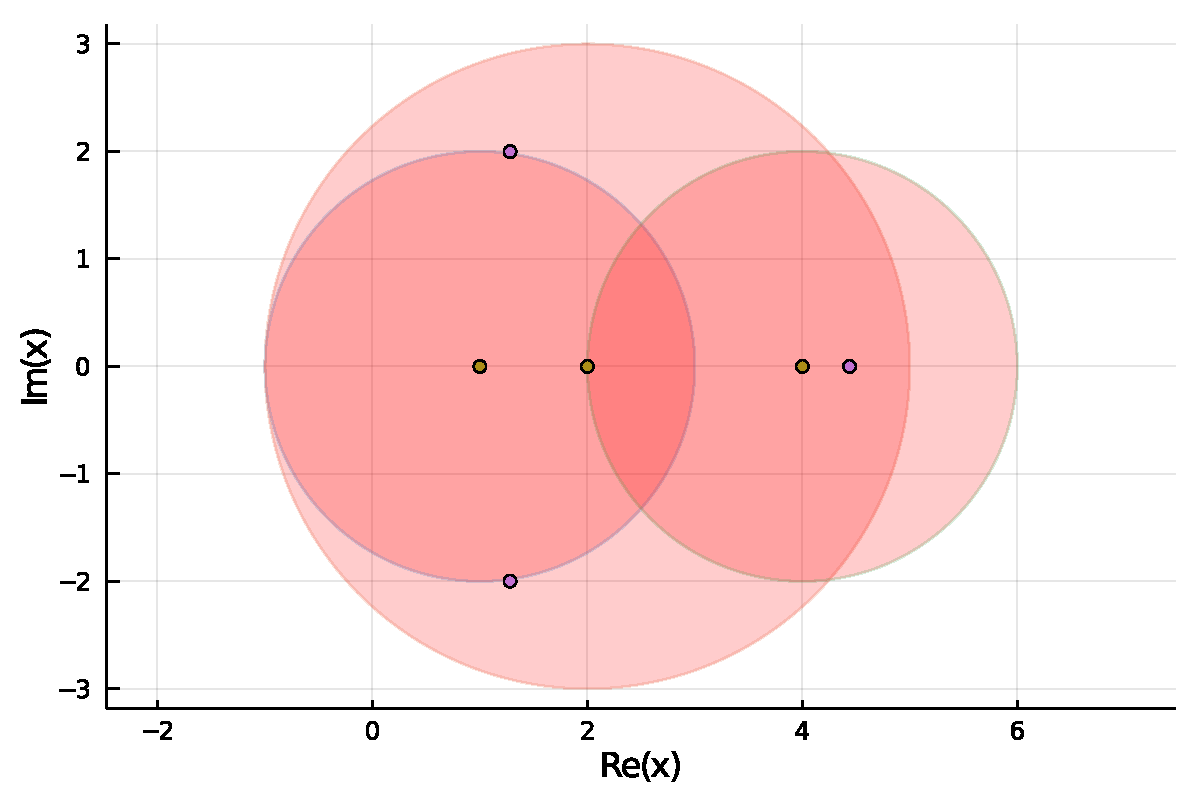
\includegraphics[width=\linewidth]{C:/Users/mfaso/OneDrive/Documents/GitHub/M3M6AppliedComplexAnalysis/output/figures/Solutions2_2_1.pdf}

\begin{itemize}
\item[3. ] \end{itemize}
Because the spectrum live in the intersection of the two estimates, the sharpest bound is

\[
\sigma(A) \subseteq B(2,3)
\]

\begin{lstlisting}
(*@\HLJLn{\ensuremath{\lambda}}@*) (*@\HLJLoB{=}@*) (*@\HLJLnf{eigvals}@*)(*@\HLJLp{(}@*)(*@\HLJLn{A}@*)(*@\HLJLp{)}@*)
(*@\HLJLn{p}@*) (*@\HLJLoB{=}@*) (*@\HLJLnf{plot}@*)(*@\HLJLp{()}@*)
(*@\HLJLnf{drawdisk!}@*)(*@\HLJLp{(}@*)(*@\HLJLni{2}@*)(*@\HLJLp{,}@*)(*@\HLJLni{3}@*)(*@\HLJLp{)}@*)
(*@\HLJLnf{scatter!}@*)(*@\HLJLp{(}@*)(*@\HLJLn{complex}@*)(*@\HLJLoB{.}@*)(*@\HLJLp{(}@*)(*@\HLJLn{\ensuremath{\lambda}}@*)(*@\HLJLp{);}@*) (*@\HLJLn{label}@*)(*@\HLJLoB{=}@*)(*@\HLJLs{"{}eigenvalues"{}}@*)(*@\HLJLp{)}@*)
(*@\HLJLnf{scatter!}@*)(*@\HLJLp{(}@*)(*@\HLJLn{complex}@*)(*@\HLJLoB{.}@*)(*@\HLJLp{(}@*)(*@\HLJLnf{diag}@*)(*@\HLJLp{(}@*)(*@\HLJLn{A}@*)(*@\HLJLp{));}@*) (*@\HLJLn{label}@*)(*@\HLJLoB{=}@*)(*@\HLJLs{"{}diagonals"{}}@*)(*@\HLJLp{,}@*)(*@\HLJLn{ratio}@*)(*@\HLJLoB{=}@*)(*@\HLJLnfB{1.0}@*)(*@\HLJLp{)}@*)
(*@\HLJLn{p}@*)
\end{lstlisting}

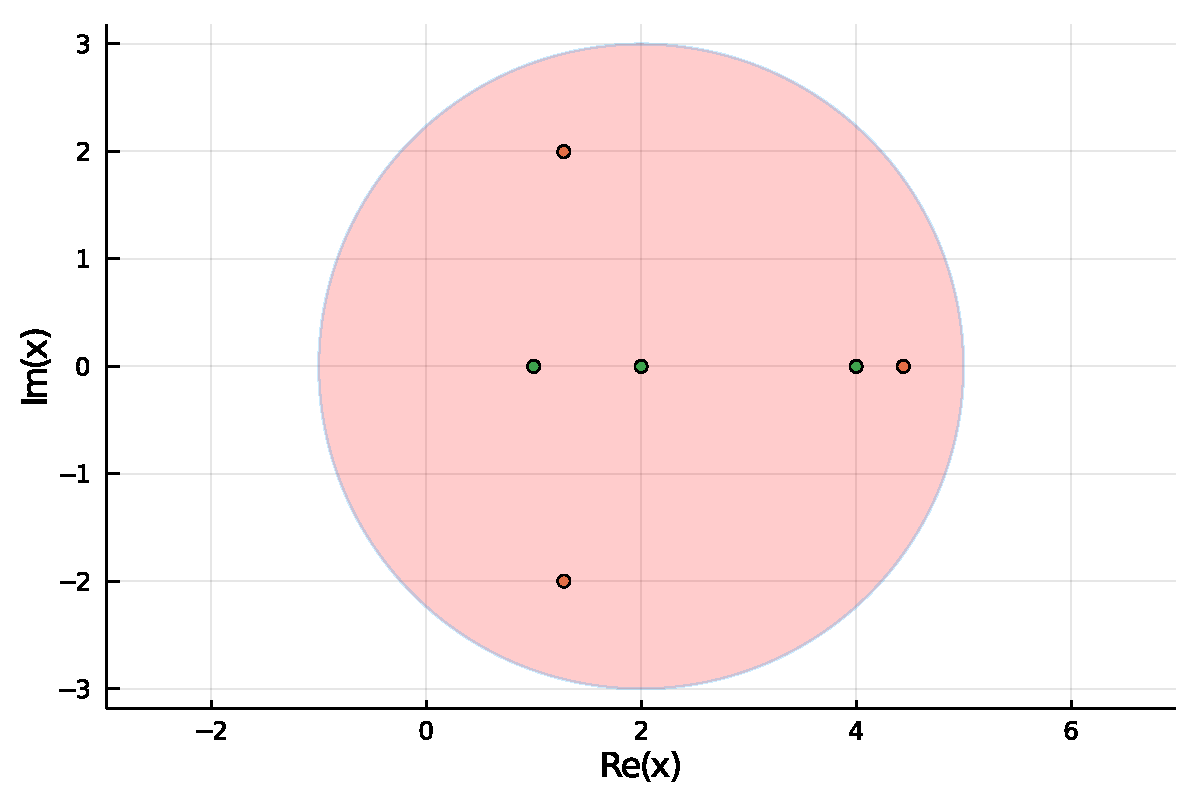
\includegraphics[width=\linewidth]{C:/Users/mfaso/OneDrive/Documents/GitHub/M3M6AppliedComplexAnalysis/output/figures/Solutions2_3_1.pdf}

Thus we can take $2 + 3 \E^{\I \theta}$ as the contour.

\subsection{Problem 2}
\begin{itemize}
\item[1. ] \end{itemize}
Note that in the scalar case $u'' = a u$ we have the solution

\[
u(t) = u_0 \cosh \sqrt{a} t + v_0 {\sinh \sqrt{a} t \over \sqrt a}
\]
Write

\[
A = Q \begin{pmatrix} \lambda_1 \\ & \ddots \\
                        && \lambda_n \end{pmatrix}  Q^\top
\]
where $\lambda_k > 0$ and then the solution has the form, where $\gamma$ is a contour surrounding the eigenvalues and to the right of zero:


\begin{align*}
    \vc u(t) &= Q \begin{pmatrix} \cosh \sqrt{\lambda_1} t \\ & \ddots \\
                        && \cosh \sqrt{\lambda_n} t  \end{pmatrix}  Q^\top \vc u_0 +
                        Q \begin{pmatrix} {\sinh \sqrt{\lambda_1} t \over \sqrt{\lambda_1}}\\ & \ddots \\
                        && {\sinh \sqrt{\lambda_n} t \over \sqrt{\lambda_n}} \end{pmatrix}  Q^\top \vc v_0 \\
              &= {1 \over 2 \pi \I} Q \begin{pmatrix}  \oint_\gamma {\cosh \sqrt{z} t  \dz \over z - \lambda_1}\\ & \ddots \\
                        &&  \oint_\gamma {\cosh \sqrt{z} t  \dz \over z - \lambda_n}\end{pmatrix}  Q^\top \vc u_0 \\
& \qquad +
                        {1 \over 2 \pi \I} Q \begin{pmatrix} \oint_\gamma {\sinh \sqrt{z} t \over \sqrt z} {\dz   \over z - \lambda_1}  \\ & \ddots \\
                        && \oint_\gamma {\sinh \sqrt{z} t \over \sqrt z} {\dz   \over z - \lambda_n}  \end{pmatrix}  Q^\top \vc v_0 \\
&= {1 \over 2 \pi \I} \oint_\gamma \cosh \sqrt{z} t   Q \begin{pmatrix}  (z - \lambda_1)^{-1}\\ & \ddots \\
                        &&    (z - \lambda_n)^{-1}\end{pmatrix}  Q^\top \vc u_0 \dz \\
&\qquad +  {1 \over 2 \pi \I} \oint_\gamma {\sinh \sqrt{z} t \over \sqrt z}   Q \begin{pmatrix}  (z - \lambda_1)^{-1}\\ & \ddots \\
                        &&    (z - \lambda_n)^{-1}\end{pmatrix}  Q^\top \vc v_0 \dz \\
&= {1 \over 2 \pi \I} \oint_\gamma \cosh \sqrt{z} t  (z I - A)^{-1} \vc u_0 \dz +  {1 \over 2 \pi \I} \oint_\gamma {\sinh \sqrt{z} t \over \sqrt z}   (z I - A)^{-1} \vc v_0 \dz
\end{align*}
Here we verify the formulae numerically:


\begin{lstlisting}
(*@\HLJLn{n}@*) (*@\HLJLoB{=}@*) (*@\HLJLni{5}@*)
(*@\HLJLn{A}@*) (*@\HLJLoB{=}@*) (*@\HLJLnf{randn}@*)(*@\HLJLp{(}@*)(*@\HLJLn{n}@*)(*@\HLJLp{,}@*)(*@\HLJLn{n}@*)(*@\HLJLp{)}@*)
(*@\HLJLn{A}@*) (*@\HLJLoB{=}@*) (*@\HLJLn{A}@*)(*@\HLJLoB{+}@*) (*@\HLJLn{A}@*)(*@\HLJLoB{{\textquotesingle}}@*) (*@\HLJLoB{+}@*) (*@\HLJLni{10}@*)(*@\HLJLn{I}@*)

(*@\HLJLn{\ensuremath{\lambda}}@*)(*@\HLJLp{,}@*) (*@\HLJLn{Q}@*) (*@\HLJLoB{=}@*) (*@\HLJLnf{eigen}@*)(*@\HLJLp{(}@*)(*@\HLJLn{A}@*)(*@\HLJLp{)}@*)
(*@\HLJLn{\ensuremath{\lambda}}@*)
\end{lstlisting}

\begin{lstlisting}
5-element Array(*@{{\{}}@*)Float64,1(*@{{\}}}@*):
  5.433025054599263
  7.14656912761484
 10.157156268543757
 11.737040975203197
 14.225630632759346
\end{lstlisting}


\begin{lstlisting}
(*@\HLJLnf{norm}@*)(*@\HLJLp{(}@*)(*@\HLJLn{A}@*) (*@\HLJLoB{-}@*) (*@\HLJLn{Q}@*)(*@\HLJLoB{*}@*)(*@\HLJLnf{Diagonal}@*)(*@\HLJLp{(}@*)(*@\HLJLn{\ensuremath{\lambda}}@*)(*@\HLJLp{)}@*)(*@\HLJLoB{*}@*)(*@\HLJLn{Q}@*)(*@\HLJLoB{{\textquotesingle}}@*)(*@\HLJLp{)}@*)
\end{lstlisting}

\begin{lstlisting}
1.9755263701875242e-14
\end{lstlisting}


Time-stepping solution:


\begin{lstlisting}
(*@\HLJLn{u\ensuremath{\_0}}@*) (*@\HLJLoB{=}@*) (*@\HLJLnf{randn}@*)(*@\HLJLp{(}@*)(*@\HLJLn{n}@*)(*@\HLJLp{)}@*)
(*@\HLJLn{v\ensuremath{\_0}}@*) (*@\HLJLoB{=}@*) (*@\HLJLnf{randn}@*)(*@\HLJLp{(}@*)(*@\HLJLn{n}@*)(*@\HLJLp{)}@*)
(*@\HLJLn{uv}@*) (*@\HLJLoB{=}@*) (*@\HLJLnf{solve}@*)(*@\HLJLp{(}@*)(*@\HLJLnf{ODEProblem}@*)(*@\HLJLp{((}@*)(*@\HLJLn{uv}@*)(*@\HLJLp{,}@*)(*@\HLJLn{{\_}}@*)(*@\HLJLp{,}@*)(*@\HLJLn{t}@*)(*@\HLJLp{)}@*) (*@\HLJLoB{->}@*) (*@\HLJLp{[}@*)(*@\HLJLn{uv}@*)(*@\HLJLp{[}@*)(*@\HLJLn{n}@*)(*@\HLJLoB{+}@*)(*@\HLJLni{1}@*)(*@\HLJLoB{:}@*)(*@\HLJLk{end}@*)(*@\HLJLp{];}@*) (*@\HLJLn{A}@*)(*@\HLJLoB{*}@*)(*@\HLJLn{uv}@*)(*@\HLJLp{[}@*)(*@\HLJLni{1}@*)(*@\HLJLoB{:}@*)(*@\HLJLn{n}@*)(*@\HLJLp{]],}@*) (*@\HLJLp{[}@*)(*@\HLJLn{u\ensuremath{\_0}}@*)(*@\HLJLp{;}@*) (*@\HLJLn{v\ensuremath{\_0}}@*)(*@\HLJLp{],}@*) (*@\HLJLp{(}@*)(*@\HLJLnfB{0.}@*)(*@\HLJLp{,}@*)(*@\HLJLnfB{2.}@*)(*@\HLJLp{));}@*) (*@\HLJLn{reltol}@*)(*@\HLJLoB{=}@*)(*@\HLJLnfB{1E-10}@*)(*@\HLJLp{);}@*)

(*@\HLJLn{t}@*) (*@\HLJLoB{=}@*) (*@\HLJLnfB{2.0}@*)
(*@\HLJLnf{uv}@*)(*@\HLJLp{(}@*)(*@\HLJLn{t}@*)(*@\HLJLp{)[}@*)(*@\HLJLni{1}@*)(*@\HLJLoB{:}@*)(*@\HLJLn{n}@*)(*@\HLJLp{]}@*)
\end{lstlisting}

\begin{lstlisting}
5-element Array(*@{{\{}}@*)Float64,1(*@{{\}}}@*):
 -837.5346933329671
 -514.9456697482184
 -211.89078614575558
 -393.65378907816563
  200.06771063707546
\end{lstlisting}


Solution via diagonalization:


\begin{lstlisting}
(*@\HLJLn{Q}@*)(*@\HLJLoB{*}@*)(*@\HLJLnf{Diagonal}@*)(*@\HLJLp{(}@*)(*@\HLJLn{cosh}@*)(*@\HLJLoB{.}@*)(*@\HLJLp{(}@*)(*@\HLJLn{sqrt}@*)(*@\HLJLoB{.}@*)(*@\HLJLp{(}@*)(*@\HLJLn{\ensuremath{\lambda}}@*)(*@\HLJLp{)}@*) (*@\HLJLoB{.*}@*) (*@\HLJLn{t}@*)(*@\HLJLp{))}@*)(*@\HLJLoB{*}@*)(*@\HLJLn{Q}@*)(*@\HLJLoB{{\textquotesingle}*}@*)(*@\HLJLn{u\ensuremath{\_0}}@*) (*@\HLJLoB{+}@*) (*@\HLJLn{Q}@*)(*@\HLJLoB{*}@*)(*@\HLJLnf{Diagonal}@*)(*@\HLJLp{(}@*)(*@\HLJLn{sinh}@*)(*@\HLJLoB{.}@*)(*@\HLJLp{(}@*)(*@\HLJLn{sqrt}@*)(*@\HLJLoB{.}@*)(*@\HLJLp{(}@*)(*@\HLJLn{\ensuremath{\lambda}}@*)(*@\HLJLp{)}@*) (*@\HLJLoB{.*}@*) (*@\HLJLn{t}@*)(*@\HLJLp{)}@*) (*@\HLJLoB{./}@*) (*@\HLJLn{sqrt}@*)(*@\HLJLoB{.}@*)(*@\HLJLp{(}@*)(*@\HLJLn{\ensuremath{\lambda}}@*)(*@\HLJLp{))}@*)(*@\HLJLoB{*}@*)(*@\HLJLn{Q}@*)(*@\HLJLoB{{\textquotesingle}*}@*)(*@\HLJLn{v\ensuremath{\_0}}@*)
\end{lstlisting}

\begin{lstlisting}
5-element Array(*@{{\{}}@*)Float64,1(*@{{\}}}@*):
 -837.534693246912
 -514.9456696991397
 -211.89078611263412
 -393.6537890228899
  200.06771061234735
\end{lstlisting}


Solution via elliptic integrals. We chose the ellipse to surround all the spectrum of our particular $A$ with eigenvalues:


\begin{lstlisting}
(*@\HLJLnf{periodic{\_}rule}@*)(*@\HLJLp{(}@*)(*@\HLJLn{n}@*)(*@\HLJLp{)}@*) (*@\HLJLoB{=}@*) (*@\HLJLni{2}@*)(*@\HLJLn{\ensuremath{\pi}}@*)(*@\HLJLoB{/}@*)(*@\HLJLn{n}@*)(*@\HLJLoB{*}@*)(*@\HLJLp{(}@*)(*@\HLJLni{0}@*)(*@\HLJLoB{:}@*)(*@\HLJLp{(}@*)(*@\HLJLn{n}@*)(*@\HLJLoB{-}@*)(*@\HLJLni{1}@*)(*@\HLJLp{)),}@*) (*@\HLJLni{2}@*)(*@\HLJLn{\ensuremath{\pi}}@*)(*@\HLJLoB{/}@*)(*@\HLJLn{n}@*)(*@\HLJLoB{*}@*)(*@\HLJLnf{ones}@*)(*@\HLJLp{(}@*)(*@\HLJLn{n}@*)(*@\HLJLp{)}@*)

(*@\HLJLk{function}@*) (*@\HLJLnf{ellipse{\_}rule}@*)(*@\HLJLp{(}@*)(*@\HLJLn{n}@*)(*@\HLJLp{,}@*) (*@\HLJLn{a}@*)(*@\HLJLp{,}@*) (*@\HLJLn{b}@*)(*@\HLJLp{)}@*)
    (*@\HLJLn{\ensuremath{\theta}}@*) (*@\HLJLoB{=}@*) (*@\HLJLnf{periodic{\_}rule}@*)(*@\HLJLp{(}@*)(*@\HLJLn{n}@*)(*@\HLJLp{)[}@*)(*@\HLJLni{1}@*)(*@\HLJLp{]}@*)
    (*@\HLJLn{a}@*)(*@\HLJLoB{*}@*)(*@\HLJLn{cos}@*)(*@\HLJLoB{.}@*)(*@\HLJLp{(}@*)(*@\HLJLn{\ensuremath{\theta}}@*)(*@\HLJLp{)}@*) (*@\HLJLoB{+}@*) (*@\HLJLn{b}@*)(*@\HLJLoB{*}@*)(*@\HLJLn{im}@*)(*@\HLJLoB{*}@*)(*@\HLJLn{sin}@*)(*@\HLJLoB{.}@*)(*@\HLJLp{(}@*)(*@\HLJLn{\ensuremath{\theta}}@*)(*@\HLJLp{),}@*) (*@\HLJLni{2}@*)(*@\HLJLn{\ensuremath{\pi}}@*)(*@\HLJLoB{/}@*)(*@\HLJLn{n}@*)(*@\HLJLoB{*}@*)(*@\HLJLp{(}@*)(*@\HLJLoB{-}@*)(*@\HLJLn{a}@*)(*@\HLJLoB{*}@*)(*@\HLJLn{sin}@*)(*@\HLJLoB{.}@*)(*@\HLJLp{(}@*)(*@\HLJLn{\ensuremath{\theta}}@*)(*@\HLJLp{)}@*) (*@\HLJLoB{+}@*) (*@\HLJLn{im}@*)(*@\HLJLoB{*}@*)(*@\HLJLn{b}@*)(*@\HLJLoB{*}@*)(*@\HLJLn{cos}@*)(*@\HLJLoB{.}@*)(*@\HLJLp{(}@*)(*@\HLJLn{\ensuremath{\theta}}@*)(*@\HLJLp{))}@*)
(*@\HLJLk{end}@*)

(*@\HLJLk{function}@*) (*@\HLJLnf{ellipse{\_}f}@*)(*@\HLJLp{(}@*)(*@\HLJLn{f}@*)(*@\HLJLp{,}@*) (*@\HLJLn{A}@*)(*@\HLJLp{,}@*) (*@\HLJLn{n}@*)(*@\HLJLp{,}@*) (*@\HLJLn{z\ensuremath{\_0}}@*)(*@\HLJLp{,}@*) (*@\HLJLn{a}@*)(*@\HLJLp{,}@*) (*@\HLJLn{b}@*)(*@\HLJLp{)}@*)
    (*@\HLJLn{z}@*)(*@\HLJLp{,}@*)(*@\HLJLn{w}@*) (*@\HLJLoB{=}@*) (*@\HLJLnf{ellipse{\_}rule}@*)(*@\HLJLp{(}@*)(*@\HLJLn{n}@*)(*@\HLJLp{,}@*)(*@\HLJLn{a}@*)(*@\HLJLp{,}@*)(*@\HLJLn{b}@*)(*@\HLJLp{)}@*)
    (*@\HLJLn{z}@*) (*@\HLJLoB{.+=}@*) (*@\HLJLn{z\ensuremath{\_0}}@*)

    (*@\HLJLn{ret}@*) (*@\HLJLoB{=}@*) (*@\HLJLnf{zero}@*)(*@\HLJLp{(}@*)(*@\HLJLn{A}@*)(*@\HLJLp{)}@*)
    (*@\HLJLk{for}@*) (*@\HLJLn{j}@*)(*@\HLJLoB{=}@*)(*@\HLJLni{1}@*)(*@\HLJLoB{:}@*)(*@\HLJLn{n}@*)
        (*@\HLJLn{ret}@*) (*@\HLJLoB{+=}@*) (*@\HLJLn{w}@*)(*@\HLJLp{[}@*)(*@\HLJLn{j}@*)(*@\HLJLp{]}@*)(*@\HLJLoB{*}@*)(*@\HLJLnf{f}@*)(*@\HLJLp{(}@*)(*@\HLJLn{z}@*)(*@\HLJLp{[}@*)(*@\HLJLn{j}@*)(*@\HLJLp{])}@*)(*@\HLJLoB{*}@*)(*@\HLJLnf{inv}@*)(*@\HLJLp{(}@*)(*@\HLJLn{z}@*)(*@\HLJLp{[}@*)(*@\HLJLn{j}@*)(*@\HLJLp{]}@*)(*@\HLJLoB{*}@*)(*@\HLJLn{I}@*) (*@\HLJLoB{-}@*) (*@\HLJLn{A}@*)(*@\HLJLp{)}@*)
    (*@\HLJLk{end}@*)
    (*@\HLJLn{ret}@*)(*@\HLJLoB{/}@*)(*@\HLJLp{(}@*)(*@\HLJLni{2}@*)(*@\HLJLn{\ensuremath{\pi}}@*)(*@\HLJLoB{*}@*)(*@\HLJLn{im}@*)(*@\HLJLp{)}@*)
(*@\HLJLk{end}@*)

(*@\HLJLn{n}@*) (*@\HLJLoB{=}@*) (*@\HLJLni{50}@*)
(*@\HLJLnf{ellipse{\_}f}@*)(*@\HLJLp{(}@*)(*@\HLJLn{z}@*) (*@\HLJLoB{->}@*) (*@\HLJLnf{cosh}@*)(*@\HLJLp{(}@*)(*@\HLJLnf{sqrt}@*)(*@\HLJLp{(}@*)(*@\HLJLn{z}@*)(*@\HLJLp{)}@*)(*@\HLJLoB{*}@*)(*@\HLJLn{t}@*)(*@\HLJLp{),}@*) (*@\HLJLn{A}@*)(*@\HLJLp{,}@*) (*@\HLJLn{n}@*)(*@\HLJLp{,}@*) (*@\HLJLnfB{10.0}@*)(*@\HLJLp{,}@*) (*@\HLJLnfB{7.0}@*)(*@\HLJLp{,}@*) (*@\HLJLnfB{2.0}@*)(*@\HLJLp{)}@*)(*@\HLJLoB{*}@*)(*@\HLJLn{u\ensuremath{\_0}}@*) (*@\HLJLoB{+}@*)
    (*@\HLJLnf{ellipse{\_}f}@*)(*@\HLJLp{(}@*)(*@\HLJLn{z}@*) (*@\HLJLoB{->}@*) (*@\HLJLnf{sinh}@*)(*@\HLJLp{(}@*)(*@\HLJLnf{sqrt}@*)(*@\HLJLp{(}@*)(*@\HLJLn{z}@*)(*@\HLJLp{)}@*)(*@\HLJLoB{*}@*)(*@\HLJLn{t}@*)(*@\HLJLp{)}@*)(*@\HLJLoB{/}@*)(*@\HLJLnf{sqrt}@*)(*@\HLJLp{(}@*)(*@\HLJLn{z}@*)(*@\HLJLp{),}@*) (*@\HLJLn{A}@*)(*@\HLJLp{,}@*) (*@\HLJLn{n}@*)(*@\HLJLp{,}@*) (*@\HLJLnfB{10.0}@*)(*@\HLJLp{,}@*) (*@\HLJLnfB{7.0}@*)(*@\HLJLp{,}@*) (*@\HLJLnfB{2.0}@*)(*@\HLJLp{)}@*)(*@\HLJLoB{*}@*)(*@\HLJLn{v\ensuremath{\_0}}@*)
\end{lstlisting}

\begin{lstlisting}
5-element Array(*@{{\{}}@*)Complex(*@{{\{}}@*)Float64(*@{{\}}}@*),1(*@{{\}}}@*):
  -837.5352753313373 - 5.3232208872848765e-14im
   -514.945940243416 - 3.0596034914807286e-15im
 -211.89087791768256 + 2.7301183311249415e-14im
  -393.6542608371482 + 5.4515179803272316e-14im
  200.06781210361413 - 1.7445181448884913e-14im
\end{lstlisting}


\begin{itemize}
\item[2. ] \end{itemize}
I put the restriction in because of the $\sqrt z$ term, which look like it is not analytic on $(-\infty,0]$. However, this restriction was NOT necessary, since in fact $\cosh \sqrt z t$ and ${\sinh \sqrt z t \over \sqrt z}$ are entire:


\begin{lstlisting}
(*@\HLJLnf{phaseplot}@*)(*@\HLJLp{(}@*)(*@\HLJLoB{-}@*)(*@\HLJLnfB{6..6}@*)(*@\HLJLp{,}@*) (*@\HLJLoB{-}@*)(*@\HLJLnfB{3..3}@*)(*@\HLJLp{,}@*) (*@\HLJLn{z}@*) (*@\HLJLoB{->}@*) (*@\HLJLnf{cosh}@*)(*@\HLJLp{(}@*)(*@\HLJLnf{sqrt}@*)(*@\HLJLp{(}@*)(*@\HLJLn{z}@*)(*@\HLJLp{)))}@*)
\end{lstlisting}

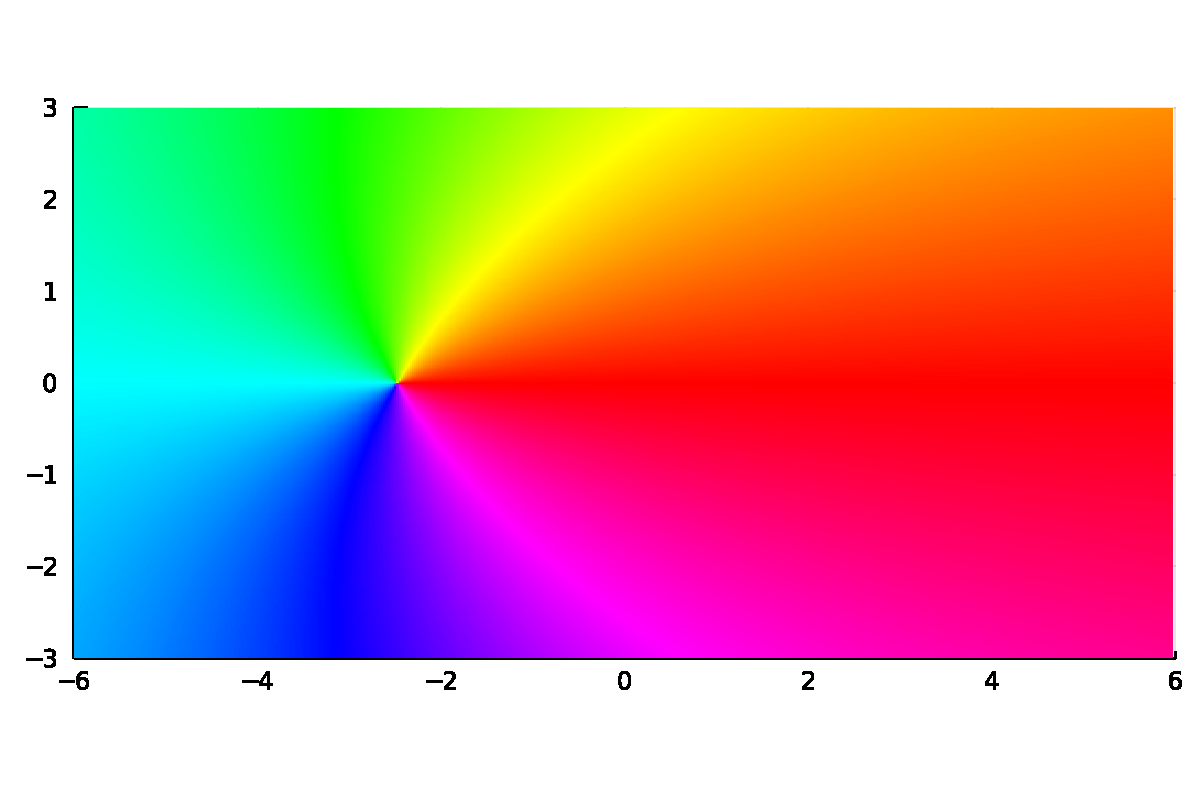
\includegraphics[width=\linewidth]{C:/Users/mfaso/OneDrive/Documents/GitHub/M3M6AppliedComplexAnalysis/output/figures/Solutions2_9_1.pdf}

\begin{lstlisting}
(*@\HLJLnf{phaseplot}@*)(*@\HLJLp{(}@*)(*@\HLJLoB{-}@*)(*@\HLJLnfB{3..3}@*)(*@\HLJLp{,}@*) (*@\HLJLoB{-}@*)(*@\HLJLnfB{3..3}@*)(*@\HLJLp{,}@*) (*@\HLJLn{z}@*) (*@\HLJLoB{->}@*) (*@\HLJLnf{sinh}@*)(*@\HLJLp{(}@*)(*@\HLJLnf{sqrt}@*)(*@\HLJLp{(}@*)(*@\HLJLn{z}@*)(*@\HLJLp{))}@*)(*@\HLJLoB{/}@*)(*@\HLJLnf{sqrt}@*)(*@\HLJLp{(}@*)(*@\HLJLn{z}@*)(*@\HLJLp{))}@*)
\end{lstlisting}

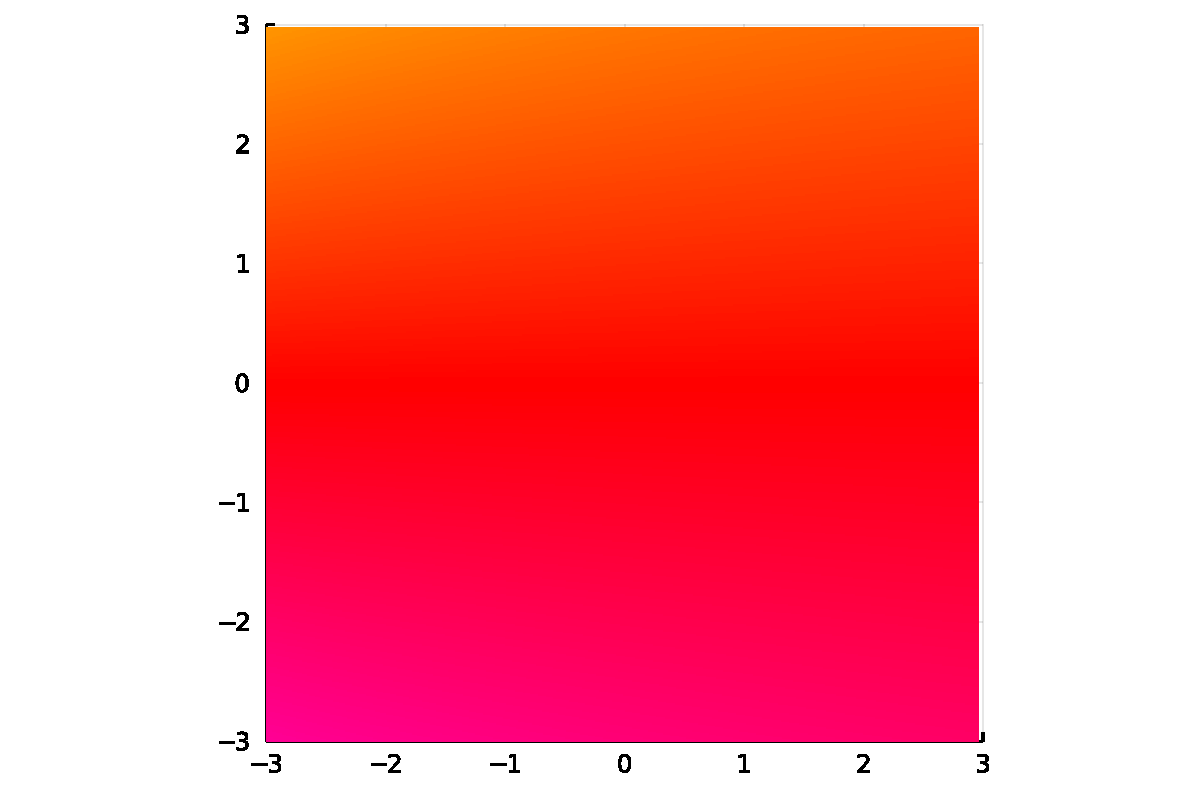
\includegraphics[width=\linewidth]{C:/Users/mfaso/OneDrive/Documents/GitHub/M3M6AppliedComplexAnalysis/output/figures/Solutions2_10_1.pdf}

This follows from Taylor series, though I prefer the following argument: we have

\[
\cosh z = {\E^{z} + \E^{-z} \over 2}
\]
hence $\cosh{\I t } = \cos t = \cosh{-\I t}$. Therefore, on the possible branch cut $\cosh \sqrt z$ is continuous (hence analytic):

\[
\cosh \sqrt{x}_+ = \cosh \I \sqrt{|x|} = \cosh -\I \sqrt{|x|} = \cosh\sqrt{x}_-
\]
Similarly,

\[
\sinh z = {\E^z - \E^{-z} \over 2}
\]
implies $\sinh{\I t} = \I \sin t = - \I \sin(-t) = -\sinh{-\I t}$, which gives us continuity:

\[
{\sinh \sqrt{x}_+ \over \sqrt{x}_+} = {\sinh \I \sqrt{|x|} \over \I \sqrt{|x|}} = {\sinh(-\I \sqrt{|x|)} \over -\I \sqrt{|x|}} ={\sinh \sqrt{x}_- \over \sqrt{x}_-}
\]
furthermore, they are both bounded at zero, hence analytic there too.

Here's a numerical example:


\begin{lstlisting}
(*@\HLJLn{n}@*) (*@\HLJLoB{=}@*) (*@\HLJLni{5}@*)
(*@\HLJLn{A}@*) (*@\HLJLoB{=}@*) (*@\HLJLnf{randn}@*)(*@\HLJLp{(}@*)(*@\HLJLn{n}@*)(*@\HLJLp{,}@*)(*@\HLJLn{n}@*)(*@\HLJLp{)}@*)
(*@\HLJLn{\ensuremath{\lambda}}@*)(*@\HLJLp{,}@*) (*@\HLJLn{V}@*) (*@\HLJLoB{=}@*) (*@\HLJLnf{eigen}@*)(*@\HLJLp{(}@*)(*@\HLJLn{A}@*)(*@\HLJLp{)}@*)
(*@\HLJLn{\ensuremath{\lambda}}@*)
\end{lstlisting}

\begin{lstlisting}
5-element Array(*@{{\{}}@*)Complex(*@{{\{}}@*)Float64(*@{{\}}}@*),1(*@{{\}}}@*):
  -2.090123104000464 + 0.0im
 -0.9325315126496077 + 0.0im
  0.3856294421143206 - 1.746951187907767im
  0.3856294421143206 + 1.746951187907767im
  1.9562214750420424 + 0.0im
\end{lstlisting}


\begin{lstlisting}
(*@\HLJLnf{norm}@*)(*@\HLJLp{(}@*)(*@\HLJLn{A}@*) (*@\HLJLoB{-}@*) (*@\HLJLn{V}@*)(*@\HLJLoB{*}@*)(*@\HLJLnf{Diagonal}@*)(*@\HLJLp{(}@*)(*@\HLJLn{\ensuremath{\lambda}}@*)(*@\HLJLp{)}@*)(*@\HLJLoB{*}@*)(*@\HLJLnf{inv}@*)(*@\HLJLp{(}@*)(*@\HLJLn{V}@*)(*@\HLJLp{))}@*)
\end{lstlisting}

\begin{lstlisting}
5.674405190697963e-15
\end{lstlisting}


\begin{lstlisting}
(*@\HLJLn{u\ensuremath{\_0}}@*) (*@\HLJLoB{=}@*) (*@\HLJLnf{randn}@*)(*@\HLJLp{(}@*)(*@\HLJLn{n}@*)(*@\HLJLp{)}@*)
(*@\HLJLn{v\ensuremath{\_0}}@*) (*@\HLJLoB{=}@*) (*@\HLJLnf{randn}@*)(*@\HLJLp{(}@*)(*@\HLJLn{n}@*)(*@\HLJLp{)}@*)
(*@\HLJLn{uv}@*) (*@\HLJLoB{=}@*) (*@\HLJLnf{solve}@*)(*@\HLJLp{(}@*)(*@\HLJLnf{ODEProblem}@*)(*@\HLJLp{((}@*)(*@\HLJLn{uv}@*)(*@\HLJLp{,}@*)(*@\HLJLn{{\_}}@*)(*@\HLJLp{,}@*)(*@\HLJLn{t}@*)(*@\HLJLp{)}@*) (*@\HLJLoB{->}@*) (*@\HLJLp{[}@*)(*@\HLJLn{uv}@*)(*@\HLJLp{[}@*)(*@\HLJLn{n}@*)(*@\HLJLoB{+}@*)(*@\HLJLni{1}@*)(*@\HLJLoB{:}@*)(*@\HLJLk{end}@*)(*@\HLJLp{];}@*) (*@\HLJLn{A}@*)(*@\HLJLoB{*}@*)(*@\HLJLn{uv}@*)(*@\HLJLp{[}@*)(*@\HLJLni{1}@*)(*@\HLJLoB{:}@*)(*@\HLJLn{n}@*)(*@\HLJLp{]],}@*) (*@\HLJLp{[}@*)(*@\HLJLn{u\ensuremath{\_0}}@*)(*@\HLJLp{;}@*) (*@\HLJLn{v\ensuremath{\_0}}@*)(*@\HLJLp{],}@*) (*@\HLJLp{(}@*)(*@\HLJLnfB{0.}@*)(*@\HLJLp{,}@*)(*@\HLJLnfB{2.}@*)(*@\HLJLp{));}@*) (*@\HLJLn{reltol}@*)(*@\HLJLoB{=}@*)(*@\HLJLnfB{1E-10}@*)(*@\HLJLp{);}@*)

(*@\HLJLn{t}@*) (*@\HLJLoB{=}@*) (*@\HLJLnfB{2.0}@*)
(*@\HLJLnf{uv}@*)(*@\HLJLp{(}@*)(*@\HLJLn{t}@*)(*@\HLJLp{)[}@*)(*@\HLJLni{1}@*)(*@\HLJLoB{:}@*)(*@\HLJLn{n}@*)(*@\HLJLp{]}@*)
\end{lstlisting}

\begin{lstlisting}
5-element Array(*@{{\{}}@*)Float64,1(*@{{\}}}@*):
 -5.239799179580709
  2.2914869877453192
 -4.1323314014116805
 -0.4246539337453159
 -1.5572758569422693
\end{lstlisting}


\begin{lstlisting}
(*@\HLJLn{V}@*)(*@\HLJLoB{*}@*)(*@\HLJLnf{Diagonal}@*)(*@\HLJLp{(}@*)(*@\HLJLn{cosh}@*)(*@\HLJLoB{.}@*)(*@\HLJLp{(}@*)(*@\HLJLn{sqrt}@*)(*@\HLJLoB{.}@*)(*@\HLJLp{(}@*)(*@\HLJLn{\ensuremath{\lambda}}@*)(*@\HLJLp{)}@*) (*@\HLJLoB{.*}@*) (*@\HLJLn{t}@*)(*@\HLJLp{))}@*)(*@\HLJLoB{*}@*)(*@\HLJLnf{inv}@*)(*@\HLJLp{(}@*)(*@\HLJLn{V}@*)(*@\HLJLp{)}@*)(*@\HLJLoB{*}@*)(*@\HLJLn{u\ensuremath{\_0}}@*) (*@\HLJLoB{+}@*)
   (*@\HLJLn{V}@*)(*@\HLJLoB{*}@*)(*@\HLJLnf{Diagonal}@*)(*@\HLJLp{(}@*)(*@\HLJLn{sinh}@*)(*@\HLJLoB{.}@*)(*@\HLJLp{(}@*)(*@\HLJLn{sqrt}@*)(*@\HLJLoB{.}@*)(*@\HLJLp{(}@*)(*@\HLJLn{\ensuremath{\lambda}}@*)(*@\HLJLp{)}@*) (*@\HLJLoB{.*}@*) (*@\HLJLn{t}@*)(*@\HLJLp{)}@*) (*@\HLJLoB{./}@*) (*@\HLJLn{sqrt}@*)(*@\HLJLoB{.}@*)(*@\HLJLp{(}@*)(*@\HLJLn{\ensuremath{\lambda}}@*)(*@\HLJLp{))}@*)(*@\HLJLoB{*}@*)(*@\HLJLnf{inv}@*)(*@\HLJLp{(}@*)(*@\HLJLn{V}@*)(*@\HLJLp{)}@*)(*@\HLJLoB{*}@*)(*@\HLJLn{v\ensuremath{\_0}}@*)
\end{lstlisting}

\begin{lstlisting}
5-element Array(*@{{\{}}@*)Complex(*@{{\{}}@*)Float64(*@{{\}}}@*),1(*@{{\}}}@*):
  -5.239799179393895 - 4.767176419984707e-16im
  2.2914869875654853 - 1.067962910696854e-15im
   -4.13233140119574 + 4.0670901795877945e-16im
 -0.4246539335944364 + 2.1951735326854606e-16im
 -1.5572758568465388 + 6.462385476705392e-16im
\end{lstlisting}


Here's the solution using an elliptic integral:


\begin{lstlisting}
(*@\HLJLn{n}@*) (*@\HLJLoB{=}@*) (*@\HLJLni{100}@*)
(*@\HLJLnf{ellipse{\_}f}@*)(*@\HLJLp{(}@*)(*@\HLJLn{z}@*) (*@\HLJLoB{->}@*) (*@\HLJLnf{cosh}@*)(*@\HLJLp{(}@*)(*@\HLJLnf{sqrt}@*)(*@\HLJLp{(}@*)(*@\HLJLn{z}@*)(*@\HLJLp{)}@*)(*@\HLJLoB{*}@*)(*@\HLJLn{t}@*)(*@\HLJLp{),}@*) (*@\HLJLn{A}@*)(*@\HLJLp{,}@*) (*@\HLJLn{n}@*)(*@\HLJLp{,}@*) (*@\HLJLnfB{0.0}@*)(*@\HLJLp{,}@*) (*@\HLJLnfB{3.0}@*)(*@\HLJLp{,}@*) (*@\HLJLnfB{3.0}@*)(*@\HLJLp{)}@*)(*@\HLJLoB{*}@*)(*@\HLJLn{u\ensuremath{\_0}}@*) (*@\HLJLoB{+}@*)
    (*@\HLJLnf{ellipse{\_}f}@*)(*@\HLJLp{(}@*)(*@\HLJLn{z}@*) (*@\HLJLoB{->}@*) (*@\HLJLnf{sinh}@*)(*@\HLJLp{(}@*)(*@\HLJLnf{sqrt}@*)(*@\HLJLp{(}@*)(*@\HLJLn{z}@*)(*@\HLJLp{)}@*)(*@\HLJLoB{*}@*)(*@\HLJLn{t}@*)(*@\HLJLp{)}@*)(*@\HLJLoB{/}@*)(*@\HLJLnf{sqrt}@*)(*@\HLJLp{(}@*)(*@\HLJLn{z}@*)(*@\HLJLp{),}@*) (*@\HLJLn{A}@*)(*@\HLJLp{,}@*) (*@\HLJLn{n}@*)(*@\HLJLp{,}@*) (*@\HLJLnfB{0.0}@*)(*@\HLJLp{,}@*) (*@\HLJLnfB{3.0}@*)(*@\HLJLp{,}@*) (*@\HLJLnfB{3.0}@*)(*@\HLJLp{)}@*)(*@\HLJLoB{*}@*)(*@\HLJLn{v\ensuremath{\_0}}@*)
\end{lstlisting}

\begin{lstlisting}
5-element Array(*@{{\{}}@*)Complex(*@{{\{}}@*)Float64(*@{{\}}}@*),1(*@{{\}}}@*):
  -5.239799179393901 - 1.6300548875775391e-15im
   2.291486987565486 + 7.4764305196881e-18im
   -4.13233140119576 + 3.6994039358526127e-16im
 -0.4246539335944406 + 1.2033882116260187e-16im
 -1.5572758568465368 + 7.477362475410658e-16im
\end{lstlisting}


\subsection{Problem 3}
\begin{itemize}
\item[1. ] \end{itemize}
We have

\[
{1 \over n} \sum_{j=0}^{n-1} g(\theta_j) = \sum_{k=0}^\infty g_k  {1 \over n} \sum_{j=0}^{n-1} \E^{\I k \theta_j}
\]
Define the $n$-th root of unity as $\omega = e^{2 \pi \I  \over n}$ (that is $\omega^n = 1$), and simplify

\[
\sum_{j=0}^{n-1} \E^{\I k \theta_j} =\sum_{j=0}^{n-1} e^{{2 \pi j \I k \over n}} =\sum_{j=0}^{n-1} \omega^{kj}= \sum_{j=0}^{n-1} (\omega^k)^j
\]
If $k$ is a multiple of $n$, then $\omega^k = 1$, and this sum is equal to $n$. If $k$ is not a multiple of $n$, use Geometric series:

\[
\sum_{j=0}^{n-1} (\omega^k)^j = {\omega^{nk} - 1 \over \omega^k -1} = {1^k - 1 \over \omega^k-1} = 0
\]
\begin{itemize}
\item[2. ] \end{itemize}
From lecture 4, we have $|f_k| \leq M_r r^{-|k|}$ for any $1 \leq r < R$, where $M_r$ is the supremum of $f$ in an annulus $\{ z : r^{-1} < |z| < r \}$. Thus from the previous part we have (using geometric series)

\[
\left| {1 \over n} \sum_{j=0}^{n-1} g(\theta_j)  - { 1\over 2 \pi}	 \int_0^{2\pi} g(\theta) \D \theta \right| \leq \sum_{K=1}^\infty |f_{Kn}| + |f_{-Kn}| \leq 2M \sum_{K=1}^\infty r^{-Kn} = 2M_r {r^{-n} \over 1 - r^{-n}}.
\]
This is an upper bound that  decays exponentially fast.

\begin{itemize}
\item[3. ] \end{itemize}
Note that $f(z) = 2 z/(4z - z^2 - 1)$ satisfies $f(\E^{\I \theta}) = g(\theta)$. This has two poles at $2 \pm \sqrt 3$:


\begin{lstlisting}
(*@\HLJLn{f}@*) (*@\HLJLoB{=}@*) (*@\HLJLn{z}@*) (*@\HLJLoB{->}@*) (*@\HLJLni{2}@*)(*@\HLJLn{z}@*)(*@\HLJLoB{/}@*)(*@\HLJLp{(}@*)(*@\HLJLni{4}@*)(*@\HLJLn{z}@*)(*@\HLJLoB{-}@*)(*@\HLJLn{z}@*)(*@\HLJLoB{{\textasciicircum}}@*)(*@\HLJLni{2}@*)(*@\HLJLoB{-}@*)(*@\HLJLni{1}@*)(*@\HLJLp{)}@*)
(*@\HLJLnf{f}@*)(*@\HLJLp{(}@*)(*@\HLJLnf{exp}@*)(*@\HLJLp{(}@*)(*@\HLJLnfB{0.1}@*)(*@\HLJLn{im}@*)(*@\HLJLp{))}@*) (*@\HLJLoB{-}@*) (*@\HLJLni{1}@*)(*@\HLJLoB{/}@*)(*@\HLJLp{(}@*)(*@\HLJLni{2}@*)(*@\HLJLoB{-}@*)(*@\HLJLnf{cos}@*)(*@\HLJLp{(}@*)(*@\HLJLnfB{0.1}@*)(*@\HLJLp{))}@*)
\end{lstlisting}

\begin{lstlisting}
1.1102230246251565e-16 + 0.0im
\end{lstlisting}


Here's a phase plot showing the location of poles:


\begin{lstlisting}
(*@\HLJLnf{phaseplot}@*)(*@\HLJLp{(}@*)(*@\HLJLoB{-}@*)(*@\HLJLnfB{5..5}@*)(*@\HLJLp{,}@*) (*@\HLJLoB{-}@*)(*@\HLJLnfB{5..5}@*)(*@\HLJLp{,}@*) (*@\HLJLn{f}@*)(*@\HLJLp{)}@*)
\end{lstlisting}

\includegraphics[width=\linewidth]{C:/Users/mfaso/OneDrive/Documents/GitHub/M3M6AppliedComplexAnalysis/output/figures/Solutions2_17_1.pdf}

\begin{lstlisting}
(*@\HLJLni{2}@*)(*@\HLJLoB{+}@*)(*@\HLJLnf{sqrt}@*)(*@\HLJLp{(}@*)(*@\HLJLni{3}@*)(*@\HLJLp{),}@*) (*@\HLJLni{2}@*)(*@\HLJLoB{-}@*) (*@\HLJLnf{sqrt}@*)(*@\HLJLp{(}@*)(*@\HLJLni{3}@*)(*@\HLJLp{),}@*) (*@\HLJLni{1}@*)(*@\HLJLoB{/}@*)(*@\HLJLp{(}@*)(*@\HLJLni{2}@*)(*@\HLJLoB{+}@*)(*@\HLJLnf{sqrt}@*)(*@\HLJLp{(}@*)(*@\HLJLni{3}@*)(*@\HLJLp{))}@*)
\end{lstlisting}

\begin{lstlisting}
(3.732050807568877, 0.2679491924311228, 0.2679491924311227)
\end{lstlisting}


Note that $2+\sqrt 3 = 1/(2-\sqrt 3)$ so in the previous result, we take $R = 2+\sqrt 3$. For any $1 \leq r < 2+\sqrt 3$ we have

\[
M_r = {2 \over 4 - r - r^{-1}}
\]
Thus we get the upper bounds

\[
    {4 \over 4 - r - r^{-1}} {r^{-n} \over 1 - r^{-n}}
\]
Let's see how sharp it is:


\begin{lstlisting}
(*@\HLJLnf{periodic{\_}rule}@*)(*@\HLJLp{(}@*)(*@\HLJLn{n}@*)(*@\HLJLp{)}@*) (*@\HLJLoB{=}@*) (*@\HLJLni{2}@*)(*@\HLJLn{\ensuremath{\pi}}@*)(*@\HLJLoB{/}@*)(*@\HLJLn{n}@*)(*@\HLJLoB{*}@*)(*@\HLJLp{(}@*)(*@\HLJLni{0}@*)(*@\HLJLoB{:}@*)(*@\HLJLp{(}@*)(*@\HLJLn{n}@*)(*@\HLJLoB{-}@*)(*@\HLJLni{1}@*)(*@\HLJLp{)),}@*) (*@\HLJLni{2}@*)(*@\HLJLn{\ensuremath{\pi}}@*)(*@\HLJLoB{/}@*)(*@\HLJLn{n}@*)(*@\HLJLoB{*}@*)(*@\HLJLnf{ones}@*)(*@\HLJLp{(}@*)(*@\HLJLn{n}@*)(*@\HLJLp{)}@*)

(*@\HLJLn{g}@*) (*@\HLJLoB{=}@*) (*@\HLJLn{\ensuremath{\theta}}@*) (*@\HLJLoB{->}@*) (*@\HLJLni{1}@*)(*@\HLJLoB{/}@*)(*@\HLJLp{(}@*)(*@\HLJLni{2}@*) (*@\HLJLoB{-}@*) (*@\HLJLnf{cos}@*)(*@\HLJLp{(}@*)(*@\HLJLn{\ensuremath{\theta}}@*)(*@\HLJLp{))}@*)

(*@\HLJLn{Q}@*) (*@\HLJLoB{=}@*) (*@\HLJLnf{sum}@*)(*@\HLJLp{(}@*)(*@\HLJLnf{Fun}@*)(*@\HLJLp{(}@*)(*@\HLJLn{g}@*)(*@\HLJLp{,}@*) (*@\HLJLni{0}@*) (*@\HLJLoB{..}@*) (*@\HLJLni{2}@*)(*@\HLJLn{\ensuremath{\pi}}@*)(*@\HLJLp{))}@*)

(*@\HLJLn{err}@*) (*@\HLJLoB{=}@*) (*@\HLJLn{Float64}@*)(*@\HLJLp{[}@*) (*@\HLJLp{(}@*)
            (*@\HLJLp{(}@*)(*@\HLJLn{\ensuremath{\theta}}@*)(*@\HLJLp{,}@*) (*@\HLJLn{w}@*)(*@\HLJLp{)}@*) (*@\HLJLoB{=}@*) (*@\HLJLnf{periodic{\_}rule}@*)(*@\HLJLp{(}@*)(*@\HLJLn{n}@*)(*@\HLJLp{);}@*)
            (*@\HLJLnf{sum}@*)(*@\HLJLp{(}@*)(*@\HLJLn{w}@*)(*@\HLJLoB{.*}@*)(*@\HLJLn{g}@*)(*@\HLJLoB{.}@*)(*@\HLJLp{(}@*)(*@\HLJLn{\ensuremath{\theta}}@*)(*@\HLJLp{))}@*) (*@\HLJLoB{-}@*) (*@\HLJLn{Q}@*)
        (*@\HLJLp{)}@*) (*@\HLJLk{for}@*) (*@\HLJLn{n}@*)(*@\HLJLoB{=}@*)(*@\HLJLni{1}@*)(*@\HLJLoB{:}@*)(*@\HLJLni{30}@*)(*@\HLJLp{];}@*)

(*@\HLJLn{N}@*) (*@\HLJLoB{=}@*) (*@\HLJLnf{length}@*)(*@\HLJLp{(}@*)(*@\HLJLn{err}@*)(*@\HLJLp{)}@*)

(*@\HLJLnf{scatter}@*)(*@\HLJLp{(}@*)(*@\HLJLn{abs}@*)(*@\HLJLoB{.}@*)(*@\HLJLp{(}@*)(*@\HLJLn{err}@*)(*@\HLJLp{),}@*) (*@\HLJLn{yscale}@*)(*@\HLJLoB{=:}@*)(*@\HLJLn{log10}@*)(*@\HLJLp{,}@*) (*@\HLJLn{label}@*)(*@\HLJLoB{=}@*)(*@\HLJLs{"{}true}@*) (*@\HLJLs{error"{}}@*)(*@\HLJLp{,}@*) (*@\HLJLn{title}@*)(*@\HLJLoB{=}@*)(*@\HLJLs{"{}Trapezium}@*) (*@\HLJLs{error}@*) (*@\HLJLs{bounds"{}}@*)(*@\HLJLp{,}@*) (*@\HLJLn{legend}@*)(*@\HLJLoB{=:}@*)(*@\HLJLn{bottomleft}@*)(*@\HLJLp{)}@*)
(*@\HLJLn{r}@*) (*@\HLJLoB{=}@*) (*@\HLJLnfB{1.1}@*)
(*@\HLJLnf{scatter!}@*)(*@\HLJLp{(}@*)(*@\HLJLni{4}@*)(*@\HLJLoB{/}@*)(*@\HLJLp{(}@*)(*@\HLJLni{4}@*)(*@\HLJLoB{-}@*)(*@\HLJLn{r}@*)(*@\HLJLoB{-}@*)(*@\HLJLnf{inv}@*)(*@\HLJLp{(}@*)(*@\HLJLn{r}@*)(*@\HLJLp{))}@*) (*@\HLJLoB{.*}@*) (*@\HLJLn{r}@*)(*@\HLJLoB{.{\textasciicircum}}@*)(*@\HLJLp{(}@*)(*@\HLJLoB{-}@*)(*@\HLJLp{(}@*)(*@\HLJLni{1}@*)(*@\HLJLoB{:}@*)(*@\HLJLn{N}@*)(*@\HLJLp{))}@*) (*@\HLJLoB{./}@*) (*@\HLJLp{(}@*)(*@\HLJLni{1}@*) (*@\HLJLoB{.-}@*) (*@\HLJLn{r}@*)(*@\HLJLoB{.{\textasciicircum}}@*)(*@\HLJLp{(}@*)(*@\HLJLoB{-}@*)(*@\HLJLp{(}@*)(*@\HLJLni{1}@*)(*@\HLJLoB{:}@*)(*@\HLJLn{N}@*)(*@\HLJLp{))),}@*) (*@\HLJLn{label}@*) (*@\HLJLoB{=}@*) (*@\HLJLs{"{}r}@*) (*@\HLJLs{=}@*) (*@\HLJLsi{{\$}r}@*)(*@\HLJLs{"{}}@*)(*@\HLJLp{)}@*)
(*@\HLJLn{r}@*) (*@\HLJLoB{=}@*) (*@\HLJLnfB{3.0}@*)
(*@\HLJLnf{scatter!}@*)(*@\HLJLp{(}@*)(*@\HLJLni{4}@*)(*@\HLJLoB{/}@*)(*@\HLJLp{(}@*)(*@\HLJLni{4}@*)(*@\HLJLoB{-}@*)(*@\HLJLn{r}@*)(*@\HLJLoB{-}@*)(*@\HLJLnf{inv}@*)(*@\HLJLp{(}@*)(*@\HLJLn{r}@*)(*@\HLJLp{))}@*) (*@\HLJLoB{.*}@*) (*@\HLJLn{r}@*)(*@\HLJLoB{.{\textasciicircum}}@*)(*@\HLJLp{(}@*)(*@\HLJLoB{-}@*)(*@\HLJLp{(}@*)(*@\HLJLni{1}@*)(*@\HLJLoB{:}@*)(*@\HLJLn{N}@*)(*@\HLJLp{))}@*) (*@\HLJLoB{./}@*) (*@\HLJLp{(}@*)(*@\HLJLni{1}@*) (*@\HLJLoB{.-}@*) (*@\HLJLn{r}@*)(*@\HLJLoB{.{\textasciicircum}}@*)(*@\HLJLp{(}@*)(*@\HLJLoB{-}@*)(*@\HLJLp{(}@*)(*@\HLJLni{1}@*)(*@\HLJLoB{:}@*)(*@\HLJLn{N}@*)(*@\HLJLp{))),}@*) (*@\HLJLn{label}@*) (*@\HLJLoB{=}@*) (*@\HLJLs{"{}r}@*) (*@\HLJLs{=}@*) (*@\HLJLsi{{\$}r}@*)(*@\HLJLs{"{}}@*)(*@\HLJLp{)}@*)
(*@\HLJLn{r}@*) (*@\HLJLoB{=}@*) (*@\HLJLni{2}@*)(*@\HLJLoB{+}@*)(*@\HLJLnf{sqrt}@*)(*@\HLJLp{(}@*)(*@\HLJLni{3}@*)(*@\HLJLp{)}@*)  (*@\HLJLoB{-}@*) (*@\HLJLnfB{0.01}@*)
(*@\HLJLnf{scatter!}@*)(*@\HLJLp{(}@*)(*@\HLJLni{4}@*)(*@\HLJLoB{/}@*)(*@\HLJLp{(}@*)(*@\HLJLni{4}@*)(*@\HLJLoB{-}@*)(*@\HLJLn{r}@*)(*@\HLJLoB{-}@*)(*@\HLJLnf{inv}@*)(*@\HLJLp{(}@*)(*@\HLJLn{r}@*)(*@\HLJLp{))}@*) (*@\HLJLoB{.*}@*) (*@\HLJLn{r}@*)(*@\HLJLoB{.{\textasciicircum}}@*)(*@\HLJLp{(}@*)(*@\HLJLoB{-}@*)(*@\HLJLp{(}@*)(*@\HLJLni{1}@*)(*@\HLJLoB{:}@*)(*@\HLJLn{N}@*)(*@\HLJLp{))}@*) (*@\HLJLoB{./}@*) (*@\HLJLp{(}@*)(*@\HLJLni{1}@*) (*@\HLJLoB{.-}@*) (*@\HLJLn{r}@*)(*@\HLJLoB{.{\textasciicircum}}@*)(*@\HLJLp{(}@*)(*@\HLJLoB{-}@*)(*@\HLJLp{(}@*)(*@\HLJLni{1}@*)(*@\HLJLoB{:}@*)(*@\HLJLn{N}@*)(*@\HLJLp{))),}@*) (*@\HLJLn{label}@*) (*@\HLJLoB{=}@*) (*@\HLJLs{"{}r}@*) (*@\HLJLs{=}@*) (*@\HLJLsi{{\$}r}@*)(*@\HLJLs{"{}}@*)(*@\HLJLp{)}@*)
\end{lstlisting}

\includegraphics[width=\linewidth]{C:/Users/mfaso/OneDrive/Documents/GitHub/M3M6AppliedComplexAnalysis/output/figures/Solutions2_19_1.pdf}


\end{document}
